\documentclass[conference]{IEEEtran}

\usepackage{amsmath,amssymb}
\usepackage{graphicx}
\usepackage{lmodern}
\usepackage{tgtermes}
\usepackage{url}

\title{Cost-Selected Parallel Decoding of Sector--Disk Erasure Codes on CPUs and GPUs}

\author{\IEEEauthorblockN{Tejas Singh Sodhi, Arnav, Advay Satish, and Dhanush Kumar}
\IEEEauthorblockA{Birla Institute of Technology and Science, Pilani\\
K K Birla Goa Campus, Goa, India}}

\begin{document}
\maketitle

\begin{abstract}
Erasure-code recovery reconstructs missing storage sectors by applying finite-field equations to surviving data. This paper evaluates CPU and CUDA decoders for Sector--Disk (SD) codes, which protect against complete-disk and additional sector failures. The decoders choose among normal recovery (apply matrices to data in sequence), matrix-first recovery (multiply coefficient matrices first), and partitioned recovery (solve independent groups before the coupled remainder). CPU optimization combines single-instruction multiple-data (SIMD) arithmetic with OpenMP threads; GPU variants use direct or table-based multiplication. Across nine 32 MiB workloads, eight-thread CPU recovery achieves 1.69$\times$--34.85$\times$ the scalar sequential baseline. Including transfers and setup, the table-based RTX 4050 decoder is 1.32$\times$--1.39$\times$ faster than eight-thread CPU recovery for GF($2^{32}$), but slower for the smaller fields. Four CPU threads outperform eight in six workloads, so these GPU gains do not establish superiority over the best CPU thread setting. CPU validation covers 7,833 feasible parameter-grid cases and 720 timed trials; separate GPU checks and all 270 CPU/GPU comparison trials pass. The results demonstrate workload-dependent benefits from arithmetic optimization and parallel execution.
\end{abstract}

\begin{IEEEkeywords}
erasure coding, Sector--Disk codes, gPPM, OpenMP, SIMD, CUDA, recovery
\end{IEEEkeywords}

\section{Introduction}
Erasure codes store data with parity so that missing sectors can be reconstructed without keeping full replicas. Recovery solves finite-field equations over the surviving data, and applying those equations to large regions can make computation a significant part of repair time. This study focuses on Sector--Disk (SD) codes, which tolerate both complete-disk failures and additional sector failures. Their parity-check equations include row-local relationships as well as equations spanning the whole stripe; this structure means some failed sectors can be recovered independently while others depend on those results \cite{li2023gppm}.

Prior work provides two ways to exploit this structure. Partitioned and Parallel Matrix (PPM) recovery separates independent failure groups and processes them concurrently \cite{li2015ppm}. Generalized PPM (gPPM) also selects between two equivalent calculation orders: first applying the parity-check matrices to data regions, or first multiplying the smaller coefficient matrices \cite{li2023gppm}. Single-instruction multiple-data (SIMD) instructions accelerate the finite-field operations within each region \cite{plank2013simd}.

This paper asks how much these optimizations contribute to an SD decoder and how GPU offloading compares with a fixed eight-thread optimized CPU configuration. We evaluate cost selection, SIMD kernels, and OpenMP parallelism on nine 32 MiB workloads, then compare eight-thread CPU recovery with direct and table-based CUDA implementations, including transfers and setup. CPU gains reach 1.69$\times$--34.85$\times$ the sequential baseline; the table GPU variant beats the eight-thread CPU only in the GF($2^{32}$) workloads. Because four threads were faster in six CPU workloads, this is not evidence that the GPU beats a thread-tuned CPU. The contribution is a reproducible implementation and evaluation on one CPU/GPU system, rather than a new code construction or distributed-scaling algorithm.

\section{Background and Related Work}
\subsection{SD-code recovery}
An SD code has $n$ disks, $r$ sector rows per disk, tolerates $m$ disk failures and $s$ additional sector failures, and uses the finite field $GF(2^w)$ of $w$-bit symbols. A stripe is the $nr$ sectors protected together; $z$ counts rows with additional sector failures. Its parity-check matrix $H$ has $mr+s$ rows. A valid stripe $B$ satisfies $HB=0$. Let $F,S$ contain the failed and surviving columns, and $B_F,B_S$ the corresponding data. For an invertible $F$,
\begin{equation}
B_F = F^{-1} S B_S.
\label{eq:recover}
\end{equation}
The normal sequence computes $S B_S$ before applying $F^{-1}$. Matrix-first computes $G=F^{-1}S$ first, then applies $G$ to the surviving data. Both recover the same sectors, but their data-region operation counts can differ \cite{li2023gppm}. SD parity equations include both row-local and stripe-wide constraints. PPM uses the row-local structure to identify independent failure groups, then recovers the coupled remainder \cite{li2015ppm}.

\subsection{Positioning among prior optimizations}
PPM introduced matrix partitioning for asymmetric codes; gPPM extended it with per-matrix sequence selection that accounts for both nonzero and non-one coefficients \cite{li2015ppm,li2023gppm}. SIMD finite-field kernels accelerate each region operation and complement this reduction in work \cite{plank2013simd}. This study keeps the SD code and parity equations fixed, and optimizes the recovery schedule and arithmetic kernels.

\section{Recovery Design}
\subsection{Cost model and selection}
For a coefficient matrix $M$, let $u(M)$ count nonzero entries and $v(M)$ count entries greater than one. A region multiply-XOR multiplies each source symbol by a field coefficient and XORs it into a destination; coefficient one requires only XOR. The estimated cost is
\begin{equation}
  C(M)=u(M)+c\,v(M),
\label{eq:cost}
\end{equation}
where $c$ estimates the additional relative cost of a non-one multiply-XOR compared with a coefficient-one XOR. For the normal and matrix-first sequences,
\begin{align}
 C_{\mathrm{normal}} &= u(S)+u(F^{-1})+c[v(S)+v(F^{-1})],\\
 C_{\mathrm{matrix}} &= u(F^{-1}S)+c\,v(F^{-1}S).
\end{align}
For PPM, the decoder sums the cheaper sequence estimate for each independent group and the remainder. It uses this partition only when its estimated cost is lower than the cheaper whole-matrix sequence. The model estimates arithmetic work, not scheduling overhead or elapsed time.

The decoder estimates $c$ per field and build by timing coefficient-one and coefficient-two operations on 256 KiB regions. It uses the multiply-XOR/XOR time ratio minus one, clamped at zero. Since this calibration is hardware-dependent, $c$ can change sequence selection across platforms.

\subsection{Partitioned and parallel execution}
Rows with exactly $m$ failed sectors have enough row-local equations to recover them independently. The decoder prepares these groups and a remainder containing the other row-local and all stripe-wide equations. OpenMP workers recover disjoint groups; a barrier ensures those outputs are ready before the remainder is decoded. The team size is capped at the number of independent groups.

The final optimization also splits the remainder's data regions into symbol-aligned byte ranges. Workers apply the same matrix-vector transformation to disjoint output ranges, avoiding write conflicts.

\subsection{SIMD region kernels}
The SIMD build dispatches at runtime with a scalar fallback. GF($2^8$) uses SSSE3 byte shuffles and nibble tables (16 bytes per vector); GF($2^{16}$) and GF($2^{32}$) use AVX2 gathers and byte-contribution tables (eight symbols per vector). The scalar comparison uses the same M3 code with SIMD disabled.

\subsection{CUDA recovery}
The GPU decoder retains matrix preparation and sequence selection on the host. Each CUDA thread computes one output field symbol, accumulating all nonzero coefficient contributions in a register. Adjacent threads process adjacent symbols, and one kernel evaluates a matrix-vector product rather than launching a kernel for each coefficient. Normal recovery needs two products; matrix-first needs one. Independent groups use separate streams and scratch buffers, and finish before the remainder starts. Each recovery transfers the stripe to the device once and copies the result back once.

The GPU scalar variant uses direct shift-and-reduce field multiplication. The table variant uses logarithm/antilogarithm tables for GF($2^8$) and GF($2^{16}$), and split-byte tables for GF($2^{32}$). Both execute many CUDA threads; ``scalar'' describes reference arithmetic, not serial GPU execution. Each variant calibrates its cost weight using sixteen interleaved coefficient-one/coefficient-two probe pairs after warm-up, each on 32,768 symbols. This is a heuristic: the fixed coefficient and restricted probe values do not represent every coefficient or data distribution, especially for split-byte multiplication.

\begin{table}[t]
\caption{CPU decoder layers in the performance comparison.}
\label{tab:layers}
\centering
\footnotesize
\begin{tabular}{c p{0.76\columnwidth}}
\hline
Layer & Decoder configuration \\
\hline
L0 & Scalar normal recovery; single-threaded reference \\
L1 & Scalar cost selection; parallel groups, serial remainder \\
L2 & L1 with SIMD region kernels \\
L3 & L2 with parallel byte ranges in the remainder \\
\hline
\end{tabular}
\end{table}

\begin{figure*}[t]
\centering
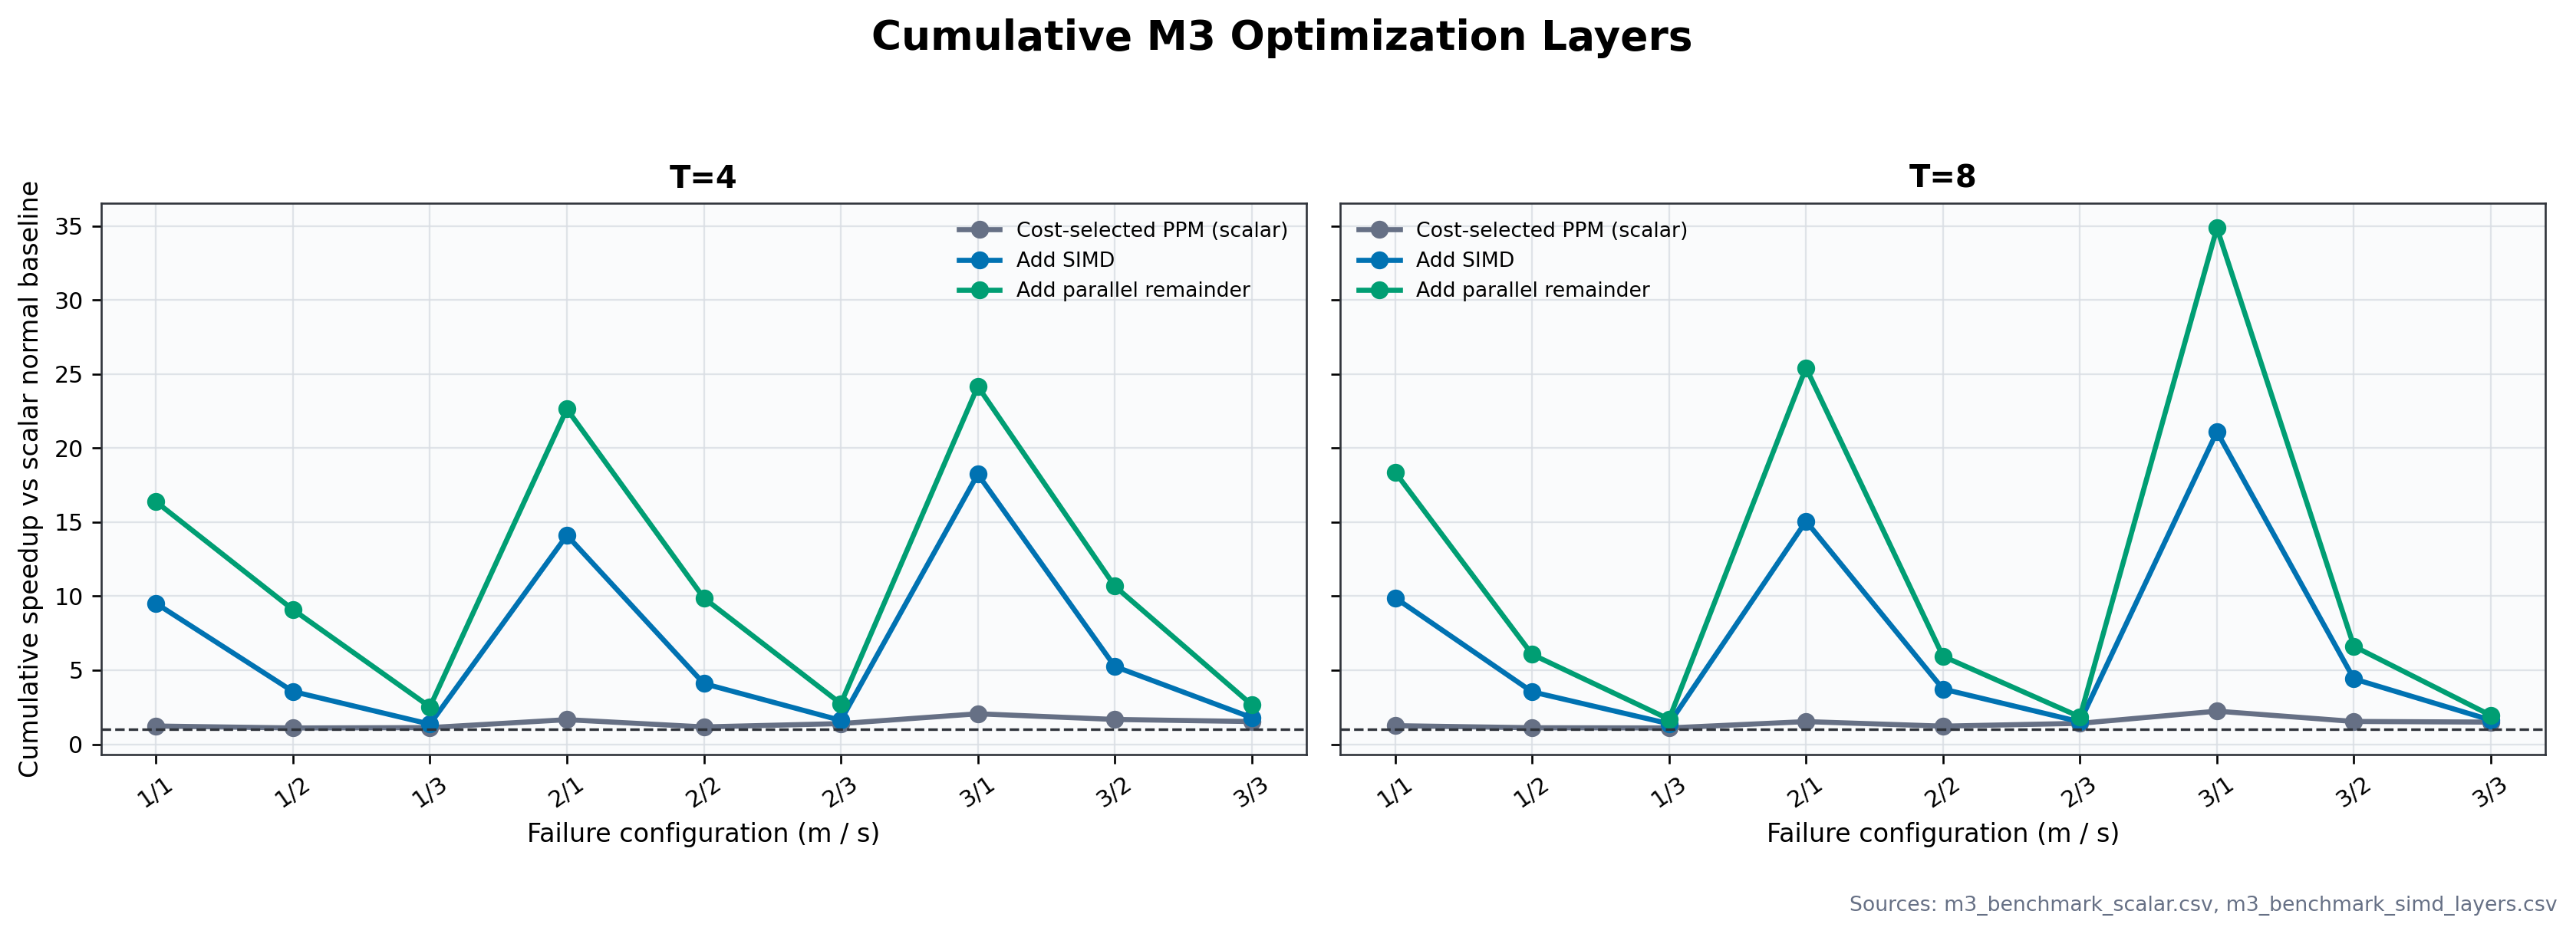
\includegraphics[width=0.96\textwidth]{../../results/milestone3/m3_cumulative_speedup.png}
\caption{Cumulative median speedup at T=4 and T=8 relative to scalar normal recovery. Curves show cost-selected scalar PPM, SIMD PPM, and SIMD PPM with a parallel remainder.}
\label{fig:layers}
\end{figure*}

\begin{table*}[t]
\caption{Single-threaded L0 median time and speedups of L1--L3 at T=8, each calculated as L0 time divided by layer time.}
\label{tab:times}
\centering
\small
\setlength{\tabcolsep}{8pt}
\renewcommand{\arraystretch}{1.15}
\begin{tabular}{cc l rrrr}
\hline
$m$ & $s$ & Field & L0 (ms) & L1 speedup & L2 speedup & L3 speedup\\
\hline
1&1&GF($2^8$) &36.031&1.25$\times$&9.89$\times$&\textbf{18.37$\times$}\\
1&2&GF($2^{16}$)&55.211&1.11$\times$&3.54$\times$&\textbf{6.07$\times$}\\
1&3&GF($2^{32}$)&45.913&1.10$\times$&1.38$\times$&\textbf{1.69$\times$}\\
2&1&GF($2^8$) &65.968&1.53$\times$&15.06$\times$&\textbf{25.42$\times$}\\
2&2&GF($2^{16}$)&82.134&1.22$\times$&3.73$\times$&\textbf{5.94$\times$}\\
2&3&GF($2^{32}$)&60.146&1.41$\times$&1.51$\times$&\textbf{1.85$\times$}\\
3&1&GF($2^8$) &99.343&2.23$\times$&21.10$\times$&\textbf{34.85$\times$}\\
3&2&GF($2^{16}$)&111.524&1.54$\times$&4.41$\times$&\textbf{6.61$\times$}\\
3&3&GF($2^{32}$)&74.373&1.49$\times$&1.63$\times$&\textbf{1.95$\times$}\\
\hline
\end{tabular}
\end{table*}

\section{Experimental Method}
\subsection{Platform and workloads}
Measurements use an Intel Core Ultra 9 185H and GCC 11.4.0 with \texttt{-O2 -fopenmp}. We test all nine $(m,s)\in\{1,2,3\}^2$ pairs at $n=r=16$, $z=1$, on a 32 MiB stripe (256 sectors of 128 KiB). For $s=1,2,3$, the fields are GF($2^8$), GF($2^{16}$), and GF($2^{32}$). Each configuration has one warm-up and ten timed recovery trials; fault injection, validation, checksums, and CSV output are excluded.

Published coefficients come from Plank's SD implementation \cite{plank2013software}. Timed failures erase disks $0,\ldots,m-1$ and sectors in row zero at columns $m,\ldots,m+s-1$, exposing 15 independent groups. Field width and sector-failure tolerance vary together; cross-field results therefore do not isolate field width alone. The previous milestone used fixed matrix-first recovery for independent groups and a normal, serial remainder.

GPU tests use an RTX 4050 Laptop GPU with 6 GB memory, driver 580.178.04, and CUDA 13.0.88 compiled with \texttt{-O2}. The CPU/GPU comparison repeats the same workloads with CPU L3 fixed at eight threads, GPU scalar, and GPU table, in that order. All share the same encoded bytes and failure layout. CPU timings are measured within this separate experiment rather than reused from the CPU-layer study; a same-run four-thread CPU comparison is not available.

Table~\ref{tab:layers} defines the four CPU layers; $T$ is the requested OpenMP thread count. L0--L1 use the scalar build; L2--L3 use the SIMD build, so L2/L1 compares complete decoders. Cumulative speedup is the L0 median divided by a layer median; incremental gain is the previous layer's median divided by the current layer's.

\subsection{Correctness and reported metrics}
Timed trials must match the saved bytes and checksum and have zero syndrome, meaning every parity equation is satisfied. The CPU sweep tests one deterministic failure layout per feasible published parameter/$z$ point, using 16-byte sectors rather than the 128 KiB timed sectors. It covers $n,r=4,\ldots,24$, $m,s=1,2,3$, and $z=1,\ldots,s$, but not every failure placement. Large-buffer SIMD behavior is checked separately in unit tests and timed recoveries.

Logical region-operation counts describe algorithmic work. Serial CPU paths count calls; parallel remainder and GPU paths derive counts from matrix nonzeros. The checks establish cross-thread consistency and agreement with each variant's warm-up count, not independent measurement of every executed operation. Useful-data throughput is non-parity bytes divided by recovery time; speedups use ratios of median end-to-end times.

GPU end-to-end timing includes host matrix preparation, device allocation, table and stripe transfers, launches, synchronization, and cleanup. Buffers and tables are recreated per recovery; CUDA startup and cost calibration occur during warm-up. Summed per-kernel CUDA-event durations are also recorded. Because streams overlap, that sum may exceed wall-clock recovery time and cannot be subtracted from it to estimate transfer time.

\section{Results}
\subsection{Correctness}
All 7,833 feasible CPU parameter-grid points pass; 105 of 7,938 parameter/$z$ combinations are infeasible. At $T=1$ and $T=4$, recovered bytes, syndromes, and operation counts agree. All 270 scalar-build and 450 SIMD-build trials pass validation. Separate GPU tests pass 12 direct/two-stage matrix checks and 64 small-stripe recoveries across all fields, both variants, and feasible failure layouts at $n=r=4$ and 24. NVIDIA Compute Sanitizer reports zero memory errors. All 270 timed CPU/GPU trials pass byte equality, checksum, and zero-syndrome checks, with logical operation counts stable across trials. The GPU tests do not reproduce the full CPU parameter-grid sweep.

\subsection{Layered performance}
Fig.~\ref{fig:layers} compares the optimization layers; Table~\ref{tab:times} gives their cumulative T=8 speedups and baseline times.

L1 improves all nine cases by 1.10$\times$--2.23$\times$ over L0. SIMD gives its largest gain in GF($2^8$): L2 reaches 21.10$\times$ over L0 and up to 9.85$\times$ over L1. In GF($2^{32}$), L2 improves on L1 by 1.07$\times$--1.26$\times$. Parallel remainder processing adds 1.20$\times$--1.86$\times$ over L2 in every T=8 case. Final speedups range from 1.69$\times$ to 34.85$\times$.

\subsection{Thread scaling}
The previous milestone's fixed PPM yielded 1.02$\times$--1.24$\times$ speedup at $T=1$ and up to 2.33$\times$ at $T=8$; three configurations slowed from four to eight threads. In M3, parallel remainder processing improves $(m,s)=(3,1)$ by 1.33$\times$ at $T=4$. However, L3 is 37\%--66\% slower at eight than at four threads in all six GF($2^{16}$)/GF($2^{32}$) workloads. Gains over L2 at a fixed thread count must not be confused with gains from increasing that count.

\subsection{GPU comparison}
Table~\ref{tab:gpu} reports the separate end-to-end CPU/GPU experiment. The table GPU variant is 1.32$\times$--1.39$\times$ faster than eight-thread CPU L3 in GF($2^{32}$), but slower in every smaller-field case. It improves on GPU scalar in six configurations by 1.08$\times$--1.23$\times$, while slowing GF($2^{16}$) recovery by factors of 1.11--1.28. These are full-decoder comparisons: separately calibrated weights can change the selected sequence and logical work, so they do not isolate table-kernel acceleration.

\begin{table}[t]
\caption{Median end-to-end recovery time (ms), including GPU transfers and setup. CPU L3 uses eight threads; speedup is its time divided by GPU table time.}
\label{tab:gpu}
\centering
\footnotesize
\setlength{\tabcolsep}{4pt}
\renewcommand{\arraystretch}{1.15}
\begin{tabular}{cc rrr r}
\hline
$m$ & $w$ & CPU L3 (8T) & GPU scalar & GPU table & Speedup\\
\hline
1&8 &2.359&22.451&20.813&0.11$\times$\\
1&16&8.887&21.428&27.386&0.32$\times$\\
1&32&26.170&22.253&19.870&\textbf{1.32$\times$}\\
2&8 &2.866&35.754&29.543&0.10$\times$\\
2&16&14.086&30.371&36.268&0.39$\times$\\
2&32&32.032&29.426&23.980&\textbf{1.34$\times$}\\
3&8 &3.107&45.353&37.567&0.08$\times$\\
3&16&18.416&36.269&40.136&0.46$\times$\\
3&32&38.682&33.979&27.915&\textbf{1.39$\times$}\\
\hline
\end{tabular}
\end{table}

Offload loses to the eight-thread CPU in the smaller-field workloads despite batched kernels. Transfer, setup, table access, and scheduling costs are included but not individually profiled. All timed variants select partitioned recovery, though their selected sequences can differ. Crucially, earlier four-thread CPU GF($2^{32}$) medians were 18.201, 21.943, and 27.914 ms---comparable to or below the GPU table results. Those separate runs cannot establish a controlled ranking, but show why the GPU gain must be restricted to the measured eight-thread comparator.

For GF($2^{32}$) at $m=1,2,3$, median summed kernel-event durations are 21.369, 59.978, and 83.212 ms for GPU scalar, versus 17.810, 35.989, and 53.776 ms for GPU table. These aggregate stream intervals describe kernel work, not the end-to-end latency in Table~\ref{tab:gpu}.

\section{Scope and Future Work}
The evaluation covers one CPU/GPU system, a fixed stripe size, nine timing configurations, and representative failure layouts. Sequential variant order, short heuristic calibration, and coupled field/failure parameters limit causal interpretation. No storage I/O, energy, or distributed scaling is measured. Priority follow-ups are a same-run CPU thread-count sweep, randomized variant order, broader calibration and failure layouts, and reuse of GPU buffers/tables across larger or batched workloads.

\section{Conclusion}
Cost selection, SIMD arithmetic, and OpenMP parallelism reach 1.69$\times$--34.85$\times$ the scalar CPU baseline at eight threads across nine 32 MiB SD workloads. Table-based GPU recovery beats the eight-thread CPU by 1.32$\times$--1.39$\times$ for GF($2^{32}$), while losing for the smaller fields. This does not establish an advantage over a thread-tuned CPU: four CPU threads outperform eight in six workloads. Correctness checks pass within the stated coverage. The practical conclusion is to evaluate algebraic work, arithmetic kernels, thread count, and offload overhead together rather than assume that additional parallelism improves recovery.

\section*{Reproducibility}
\begingroup\raggedright
CPU commands are \texttt{make m3-sweep} and \texttt{make m3-benchmark}; CUDA commands are \texttt{make gpu-test}, \texttt{make gpu-benchmark}, and \texttt{make gpu-plots}. Raw CPU timings are in \url{results/m3_benchmark_scalar.csv} and \url{results/m3_benchmark_simd_layers.csv}; GPU comparison trials are in \url{results/milestone_gpu/gpu_benchmark.csv}.
\par\endgroup

\begin{thebibliography}{00}
\bibitem{li2023gppm}
S. Li, Q. Cao, S. Wan, W. Xia, and C. Xie, ``gPPM: A generalized matrix operation and parallel algorithm to accelerate the encoding/decoding process of erasure codes,'' \emph{ACM Trans. Archit. Code Optim.}, vol. 20, no. 4, Art. no. 51, Dec. 2023, doi: 10.1145/3625005.

\bibitem{li2015ppm}
S. Li, Q. Cao, S. Wan, W. Zhang, C. Xie, X. He, and P. Subedi, ``PPM: A partitioned and parallel matrix algorithm to accelerate encoding/decoding process of asymmetric parity erasure codes,'' in \emph{Proc. 44th Int. Conf. Parallel Processing (ICPP)}, 2015, pp. 460--469, doi: 10.1109/ICPP.2015.55.

\bibitem{plank2013simd}
J. S. Plank, K. M. Greenan, and E. L. Miller, ``Screaming fast Galois field arithmetic using Intel SIMD instructions,'' in \emph{Proc. 11th USENIX Conf. File and Storage Technologies (FAST)}, 2013.

\bibitem{plank2013software}
J. S. Plank, ``Open source encoder and decoder for SD erasure codes,'' University of Tennessee, Tech. Rep. UT-CS-13-704, Jan. 2013. [Online]. Available: \url{https://web.eecs.utk.edu/~jplank/plank/papers/CS-13-704.html}

\end{thebibliography}

\end{document}
